\documentclass{article}
\usepackage{tikz}
\usetikzlibrary{arrows.meta,positioning,calc,shapes.geometric}
\pagestyle{empty}
\begin{document}
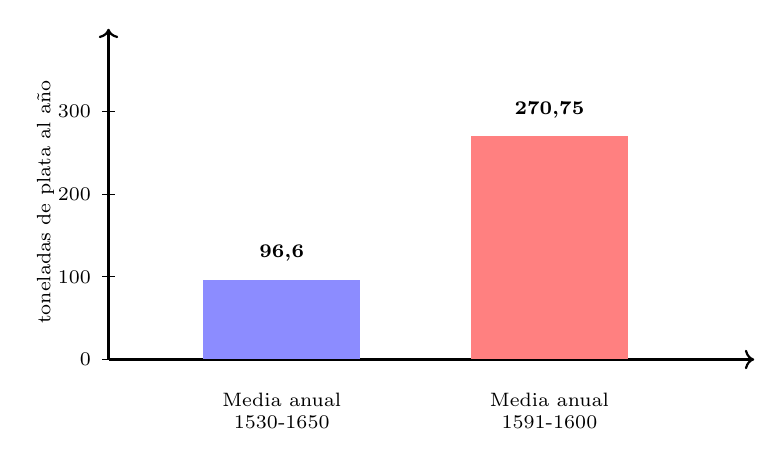
\begin{tikzpicture}
\tikzset{every node/.append style={align=center}}

\draw[->, thick] (0,0) -- (0,4.2); \draw[->, thick] (0,0) -- (8.2,0);
\node[font=\scriptsize, rotate=90] at (-0.8,2.0) {toneladas de plata al año};
\foreach \y/\l in {0/0,1.05/100,2.1/200,3.15/300} { \draw (-0.08,\y) -- (0.08,\y); \node[font=\scriptsize, anchor=east] at (-0.1,\y) {\l}; }
\fill[blue!45] (1.2,0) rectangle (3.2,1.015);
\fill[red!50] (4.6,0) rectangle (6.6,2.843);
\node[font=\scriptsize, align=center] at (2.2,-0.65) {Media anual\\1530-1650};
\node[font=\scriptsize, align=center] at (5.6,-0.65) {Media anual\\1591-1600};
\node[font=\scriptsize\bfseries] at (2.2,1.35) {96,6};
\node[font=\scriptsize\bfseries] at (5.6,3.17) {270,75};

\end{tikzpicture}
\end{document}
